% DO NOT COMPILE THIS FILE DIRECTLY!
% This is included by the other .tex files.

\begin{frame}[t,plain]
\titlepage
\end{frame}

\begin{frame}
    \frametitle{Content of the presentation}
    \begin{itemize}
        \item What problems are we trying to tackle
        \item MISP Workflows overview
        \item Design of the system \& how can it be extended
    \end{itemize}
\end{frame}

\begin{frame}
    \frametitle{What problems are we trying to tackle}
    \begin{itemize}
        \item Initial idea came from GeekWeek7.5
        \begin{center}
            
\includegraphics[width=0.5\linewidth]{pictures/geekweek75.jpg}
        \end{center}
        \item Experienced users wanted to have a way to trigger actions and to modify to behavior of MISP
        \item Use-cases:
        \begin{itemize}
            \item Prevent publication of event not meeting some criterias
            \item Enrich event before the publication takes place
        \end{itemize}
    \end{itemize}
\end{frame}

\begin{frame}
    \frametitle{Simplistic overview}
    \begin{enumerate}
        \item User/API Interraction
        \item MISP handles the request
        \item MISP executes workflows listening to the trigger
    \end{enumerate}
\end{frame}

\begin{frame}
    \frametitle{Terminology}
    \begin{enumerate}
        \item \textbf{workflow}: Sequence of actions to be executed
        \item \textbf{execution path}: A path composed of actions to be executed sequentially
        \item \textbf{trigger}: Starting point of an \texttt{execution path}. Triggers are called when specific action are done by MISP
    \end{enumerate}
    \begin{center}
        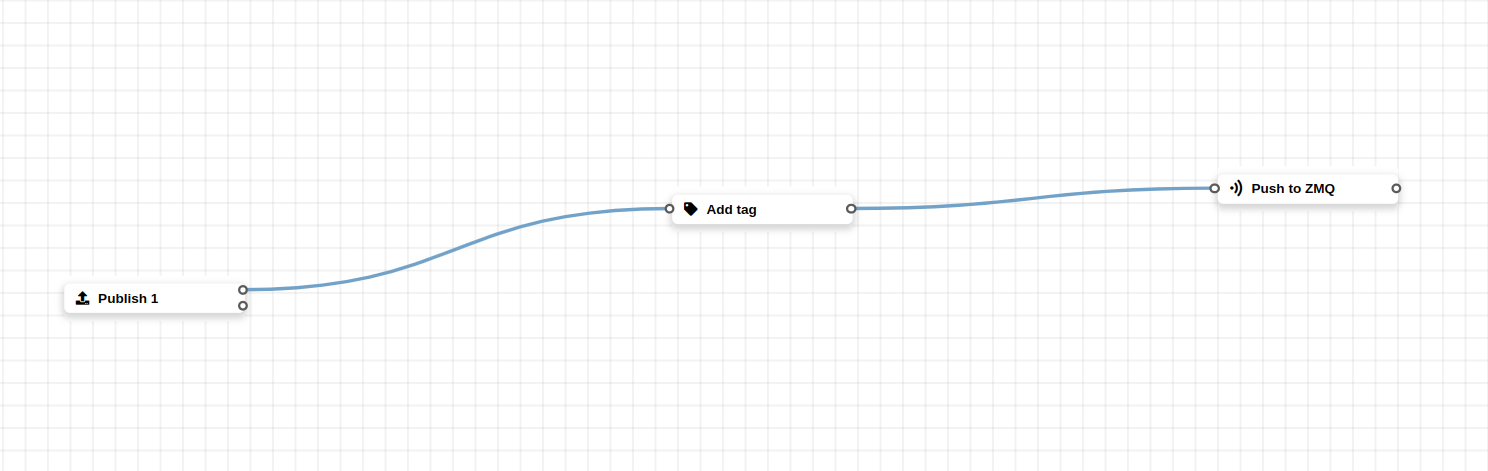
\includegraphics[width=1.0\linewidth]{pictures/workflow-view.png}
    \end{center}
\end{frame}

\begin{frame}
    \frametitle{Workflow execution}
    \begin{enumerate}
        \item A trigger is called
        \item Collect workflows listening to called trigger
        \item Execute workflows in the saved order
    \end{enumerate}
    \begin{center}
        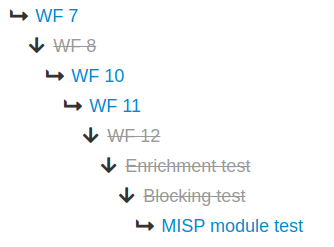
\includegraphics[width=0.5\linewidth]{pictures/execution-order-1.png}
    \end{center}
\end{frame}

\begin{frame}
    \frametitle{Execution Paths}
    Currently 2 types of execution path:
    \vspace{0.5em}
    \begin{itemize}
        \item {\bf Blocking}: Execution is stoped in case of error
        \begin{itemize}
            \item Current workflow's blocking execution path is {\bf stopped}
            \item Any other blocking path of next workflows {\bf will not be executed}
        \end{itemize}
        \vspace{0.5em}
        \item {\bf Non-blocking}/Deferred: Stop execution for current path only
        \begin{itemize}
            \item Current execution path is {\bf stopped}
            \item {\bf Resume} execution of remaining paths
            \item Paths from other workflow will be {\bf executed}
        \end{itemize}
    \end{itemize}
\end{frame}

\begin{frame}
    \frametitle{Execution Order and Execution Types}
    \begin{itemize}
        \item \textbf{Blocking} paths from all workflows are executed first in the saved order
        \item If any blocking executions failed, the action that called the trigger will \textbf{be stopped}
        \item \textbf{Parallel/Deferred} paths from all workflows are executed. The order is irrelevant
    \end{itemize}

    \begin{center}
        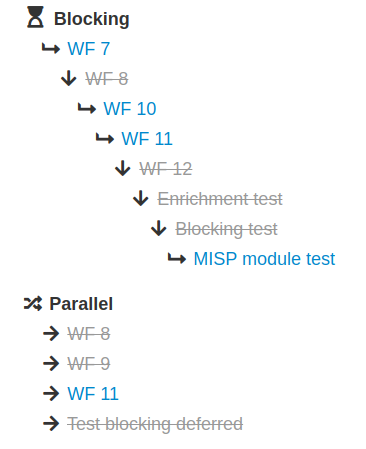
\includegraphics[width=0.35\linewidth]{pictures/execution-order-2.png}
        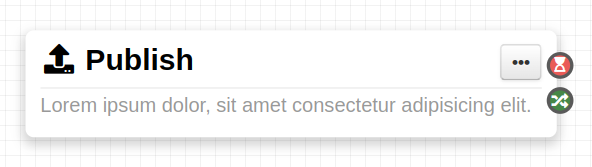
\includegraphics[width=0.40\linewidth]{pictures/trigger-outputs.png}
    \end{center}
\end{frame}

\begin{frame}
    \frametitle{Publishing example}
    Example:
    \begin{enumerate}
        \item An Event is published
        \item MISP starts the publishing process
        \item MISP executes a workflow listening to the trigger
        \begin{itemize}
            \item {\bf execution success}: Proceed publishing
            \item {\bf execution failure}: Stop publishing, log the reason and report the failure to the user
        \end{itemize}
    \end{enumerate}
\end{frame}

\begin{frame}
    \frametitle{Execution context}
    \begin{itemize}
        \item Workflow can be triggered by any users
        \item However, the user for which the workflow executes is the workflow creator
        \item This is to make sure users with a higher privilege will have their workflow correctly executed
    \end{itemize}
\end{frame}

\begin{frame}
    \frametitle{Workflow modules}
    \begin{center}
        
\includegraphics[width=0.5\linewidth]{pictures/module-type.png}
    \end{center}
    \begin{itemize}
        \item 3 types of modules
        \begin{itemize}
            \item \texttt{trigger}: Entry point of the execution
            \begin{itemize}
                \item Event publish, email about to be sent, feed data about to be saved, ...
            \end{itemize}
            \item \texttt{logic}: Allow to redirect the execution flow.
            \begin{itemize}
                \item IF condition, fork the blocking execution into a non-blocking one, ...
            \end{itemize}
            \item \texttt{action}: Modules that can modify data, prevent execution or perform additional actions
            \begin{itemize}
                \item Publish to ZMQ, perform enrichments, block the execution, ...
            \end{itemize}
        \end{itemize}
    \end{itemize}
\end{frame}

\begin{frame}
    \frametitle{Workflow modules}
    \begin{itemize}
        \item \texttt{action} modules can be from 2 sources
        \begin{itemize}
            \item \texttt{\scriptsize app/Model/WorkflowModules/action/[module\_name].php}
            \begin{itemize}
                \item Written in PHP
                \item They can use MISP's built-in functionalities (restsearch, enrichment, push to zmq, ...)
                \item Faster and easier to interact with for those having internal knowledge of MISP
            \end{itemize}
            \item \texttt{From the misp-module service} 
            \begin{itemize}
                \item Written in Python
                \item They can use any python libraries
                \item Easier to write
                \item New module type \texttt{action}
            \end{itemize}
        \end{itemize}
        \item Both systems are \textbf{plug-and-play}
    \end{itemize}
\end{frame}

\begin{frame}
    \frametitle{Creating a workflow with the editor}
    \begin{enumerate}
        \item Drag a \texttt{trigger} module from the side panel to the canvas
        \item Drag an \texttt{action} module from the side panel to the canvas
        \item From the \texttt{trigger} output, drag an arrow into the \texttt{action} input (left side)
        \begin{itemize}
            \item You can choose between a \texttt{blocking} and \texttt{non-blocking} execution path by using the associated trigger output
        \end{itemize}
    \end{enumerate}
    \begin{center}
        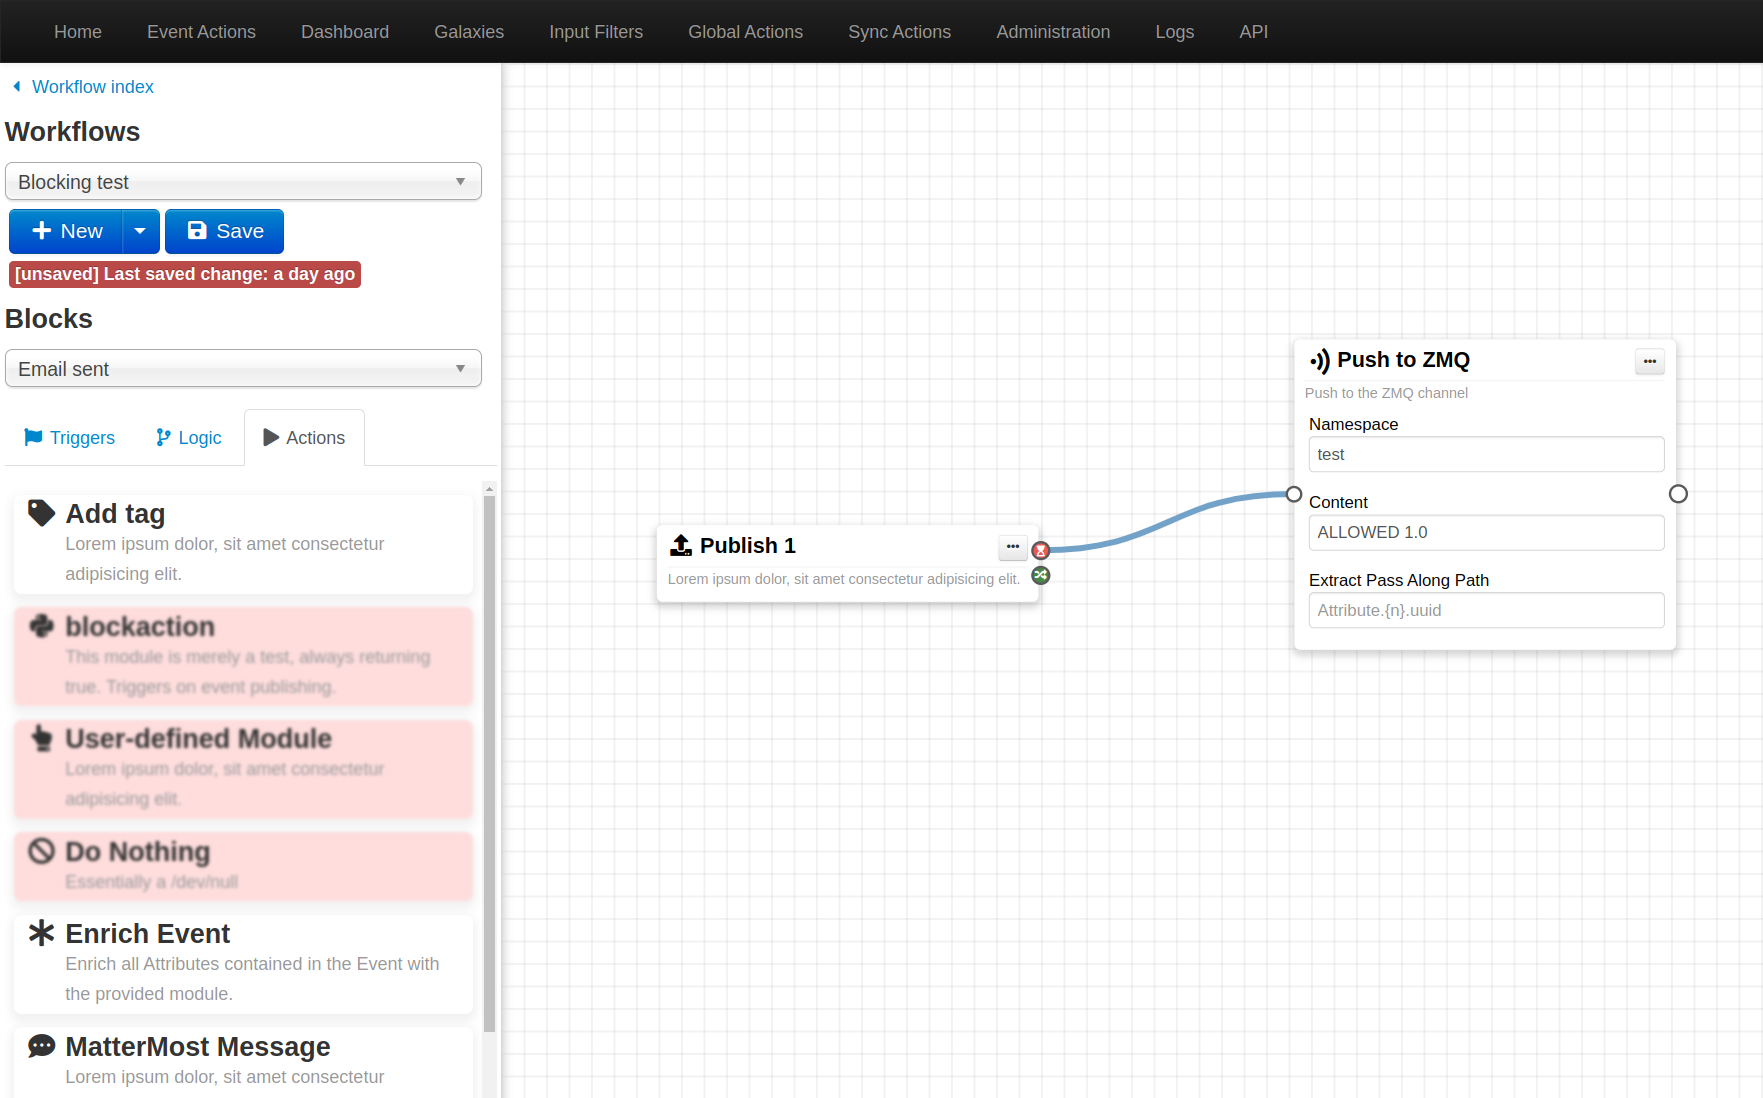
\includegraphics[width=1.0\linewidth]{pictures/editor-1.png}
    \end{center}
\end{frame}

\begin{frame}
    \frametitle{Working with the editor}
    Operations not allowed
    \begin{itemize}
        \item Create an execution loop
    \end{itemize}
    \begin{center}
        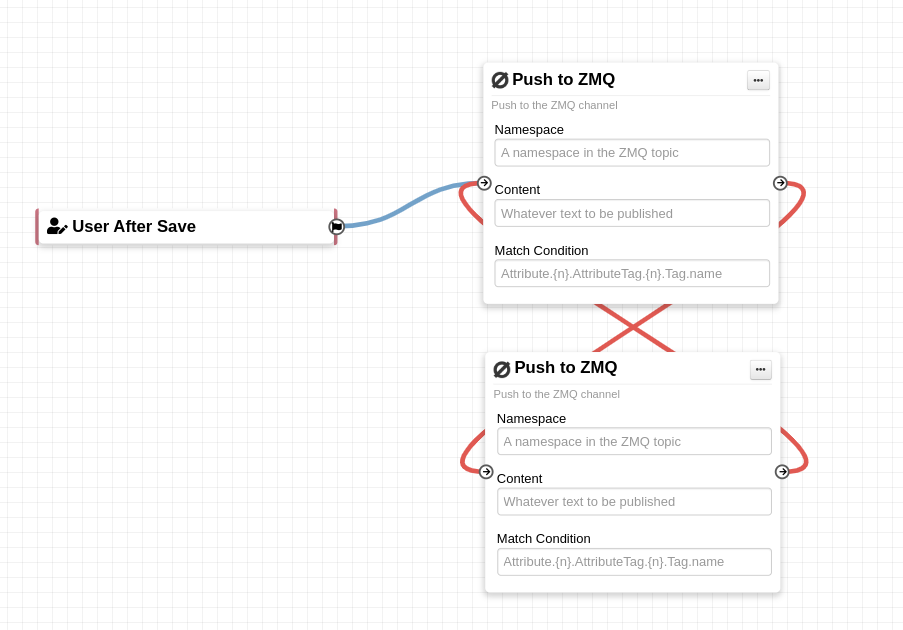
\includegraphics[width=0.7\linewidth]{pictures/editor-not-allowed-1.png}
    \end{center}
    \begin{itemize}
        \item Use the same trigger twice
    \end{itemize}
\end{frame}

\section{Learning by examples}
\begin{frame}
    \frametitle{Workflow example 1}
    \begin{center}
        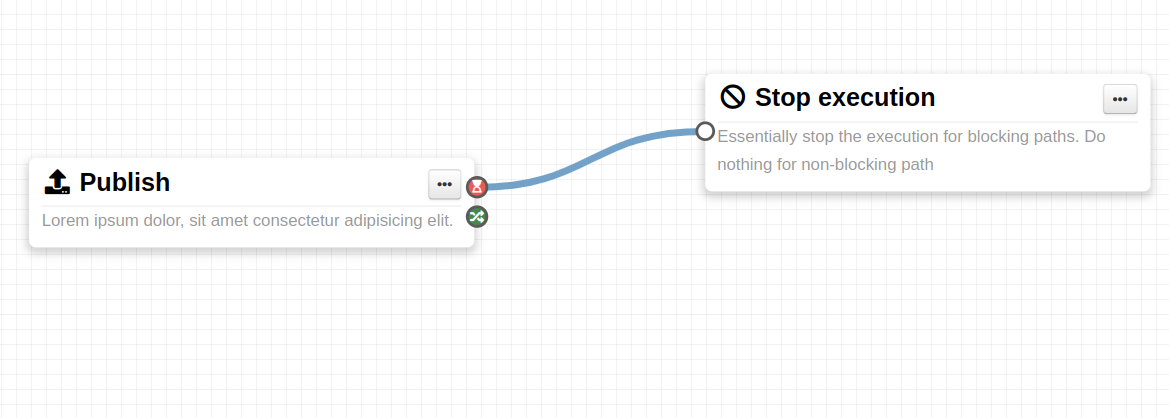
\includegraphics[width=0.9\linewidth]{pictures/example-1.png}
    \end{center}

    \begin{enumerate}
        \item Will the next blocking path (from another workflow) be executed?
    \end{enumerate}
\end{frame}
\begin{frame}
    \frametitle{Workflow example 1: Answers}
    \begin{center}
        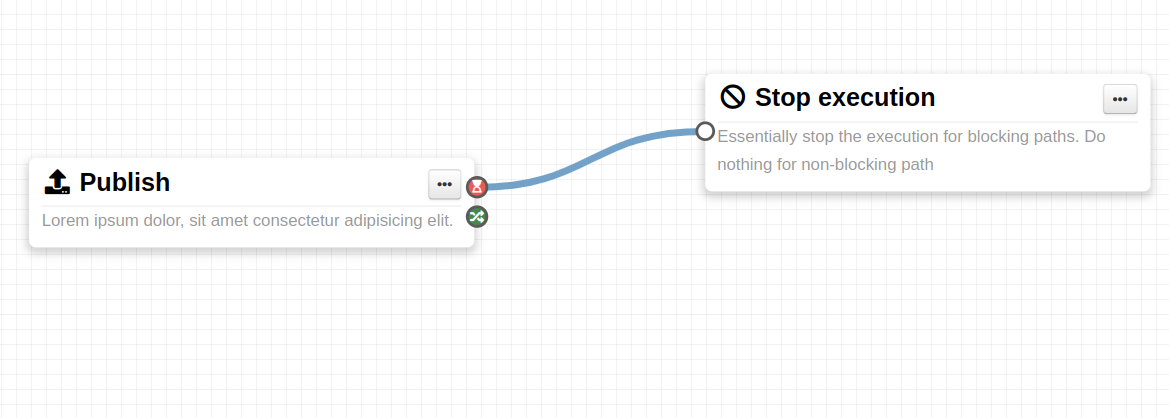
\includegraphics[width=0.9\linewidth]{pictures/example-1.png}
    \end{center}

    \begin{enumerate}
        \item Will the next blocking path (from another workflow) be executed?
        \begin{itemize}
            \item \textbf{No}. We are in a blocking path. As the execution has been stopped, no other blocking paths will be executed.
        \end{itemize}
    \end{enumerate}
\end{frame}

\begin{frame}
    \frametitle{Workflow example 2}
    \begin{center}
        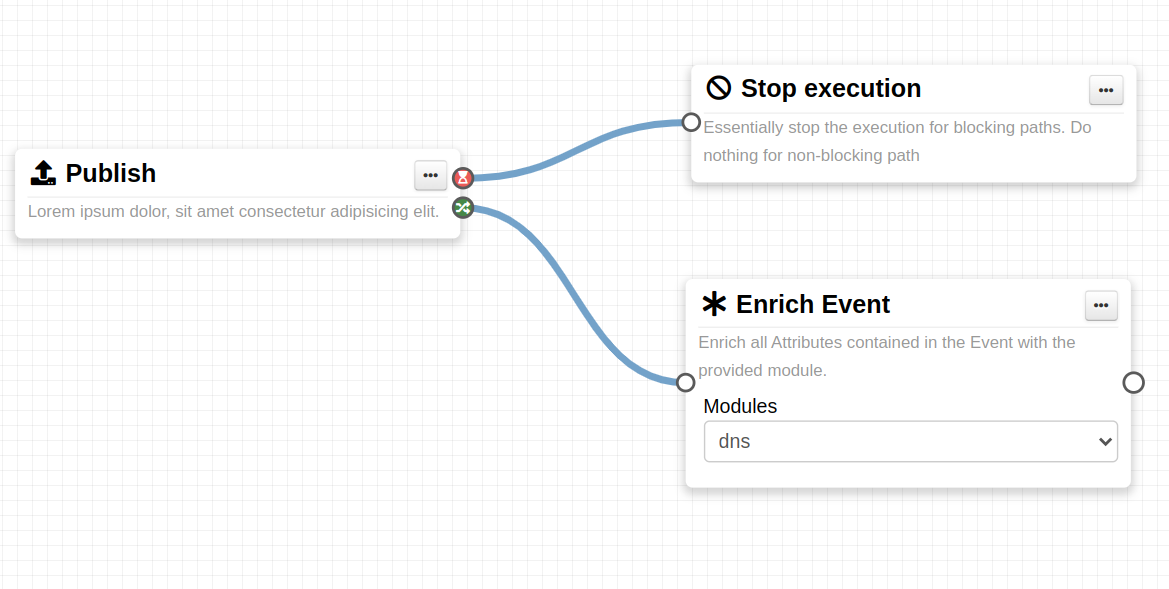
\includegraphics[width=0.9\linewidth]{pictures/example-2.png}
    \end{center}

    \begin{enumerate}
        \item Will the next blocking path (from another workflow) be executed?
        \item Will \texttt{Enrich Event} module be executed?
    \end{enumerate}
\end{frame}
\begin{frame}
    \frametitle{Workflow example 2: Answers}
    \begin{center}
        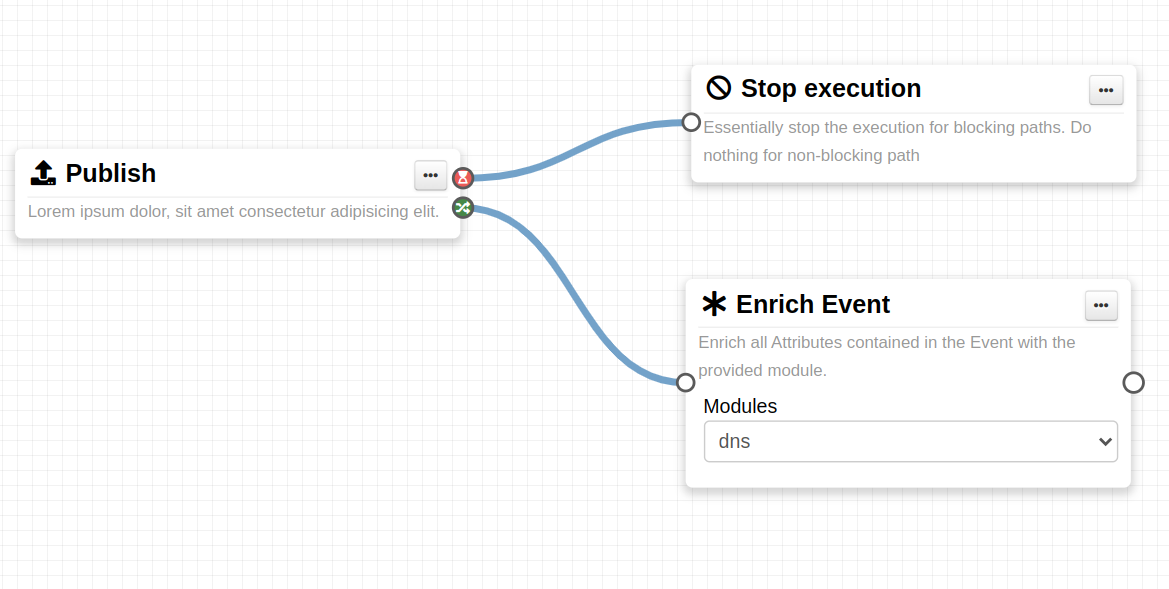
\includegraphics[width=0.7\linewidth]{pictures/example-2.png}
    \end{center}

    \begin{enumerate}
        \item Will the next blocking path (from another workflow) be executed?
        \begin{itemize}
            \item \textbf{No}. Same reason that before
        \end{itemize}
        \item Will \texttt{Enrich Event} module be executed?
        \begin{itemize}
            \item \textbf{Yes}. The module is in the non-blocking path. Regardless of the result of the blocking path, it will be executed.
        \end{itemize}
    \end{enumerate}
\end{frame}

\begin{frame}
    \frametitle{Workflow example 3}
    \begin{center}
        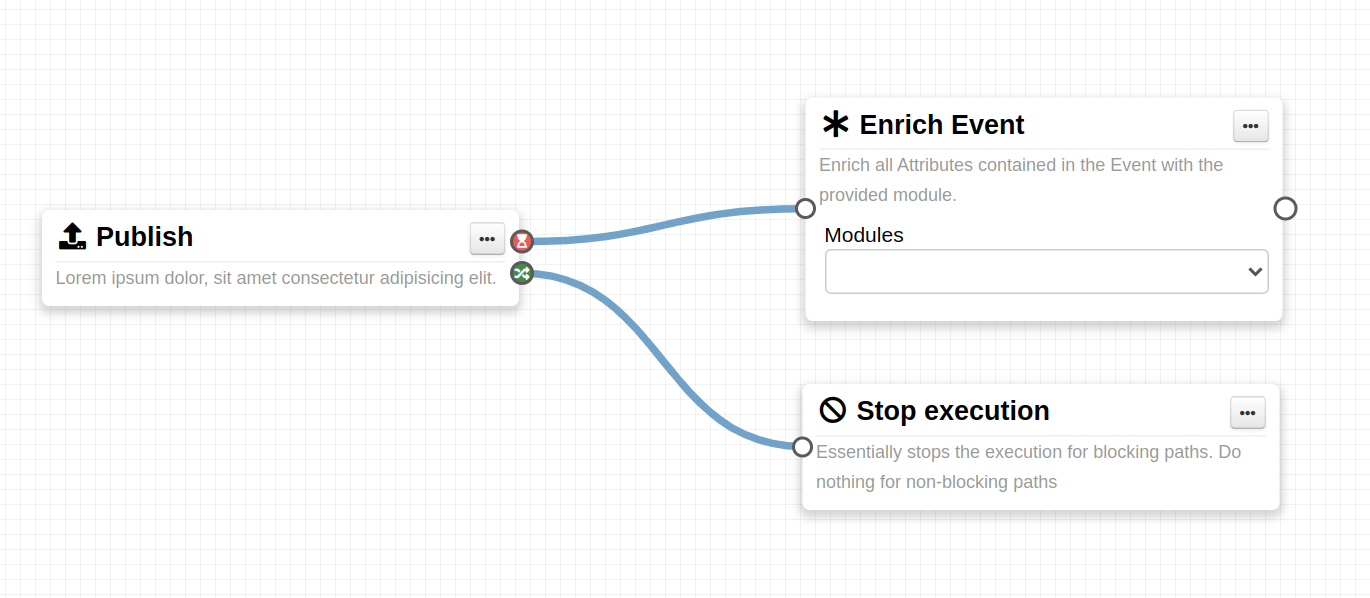
\includegraphics[width=0.9\linewidth]{pictures/example-3.png}
    \end{center}

    \begin{enumerate}
        \item Will \texttt{Enrich Event} module be executed?
        \item Will the next blocking path (from another workflow) be executed?
    \end{enumerate}
\end{frame}

\begin{frame}
    \frametitle{Workflow example 3: Answers}
    \begin{center}
        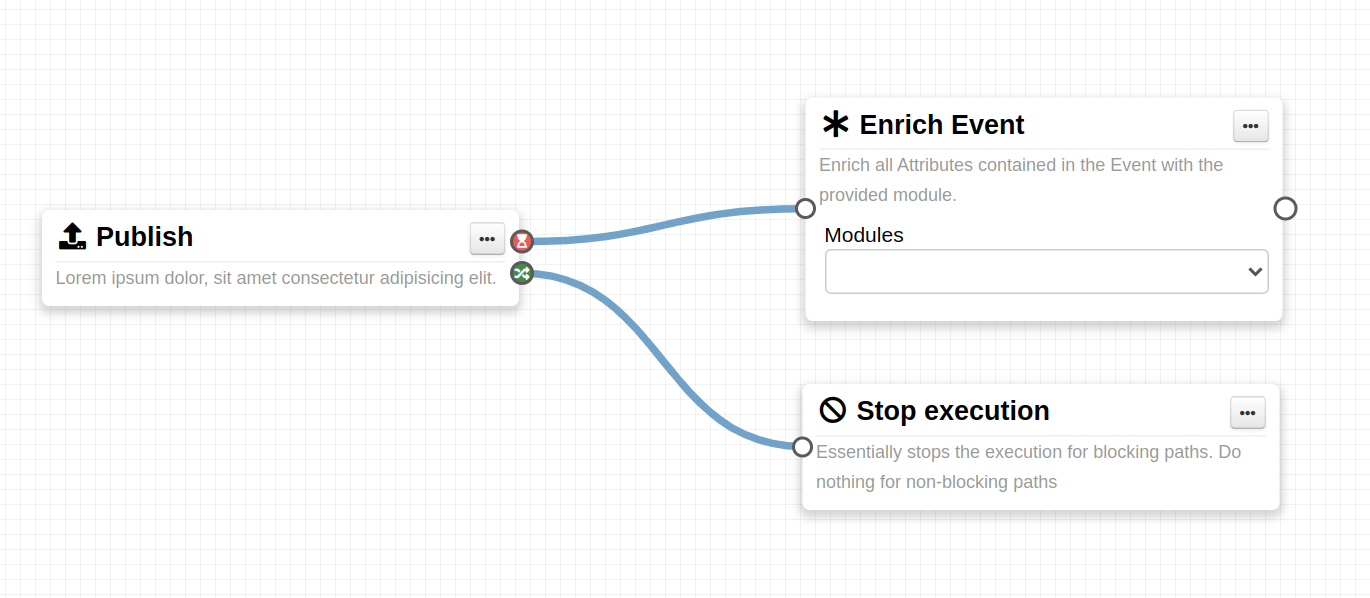
\includegraphics[width=0.55\linewidth]{pictures/example-3.png}
    \end{center}

    \begin{enumerate}
        \item Will \texttt{Enrich Event} module be executed?
        \begin{itemize}
            \item \textbf{Yes}
            \item The blocking path is executed before the non-blocking one
            \item The result of the non-blocking path has no influence on the blocking one
        \end{itemize}
        \item Will the next blocking path (from another workflow) be executed?
        \begin{itemize}
            \item \textbf{Yes}
            \item The blocking path is executed before the non-blocking one
            \item The result of the non-blocking path has no influence the execution of other workflows
        \end{itemize}
    \end{enumerate}
\end{frame}

\begin{frame}
    \frametitle{Workflow example 4}
    \begin{center}
        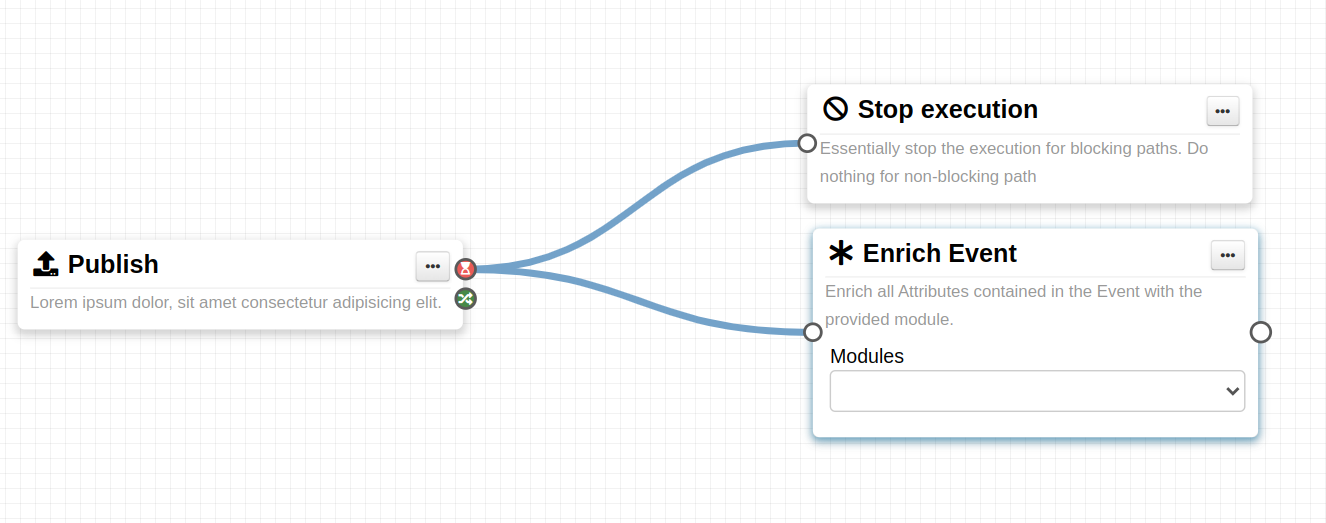
\includegraphics[width=0.9\linewidth]{pictures/example-4.png}
    \end{center}
    \begin{enumerate}
        \item Will \texttt{Enrich Event} module be executed?
    \end{enumerate}
\end{frame}


\begin{frame}
    \frametitle{Workflow example 4: Answers}
    \begin{center}
        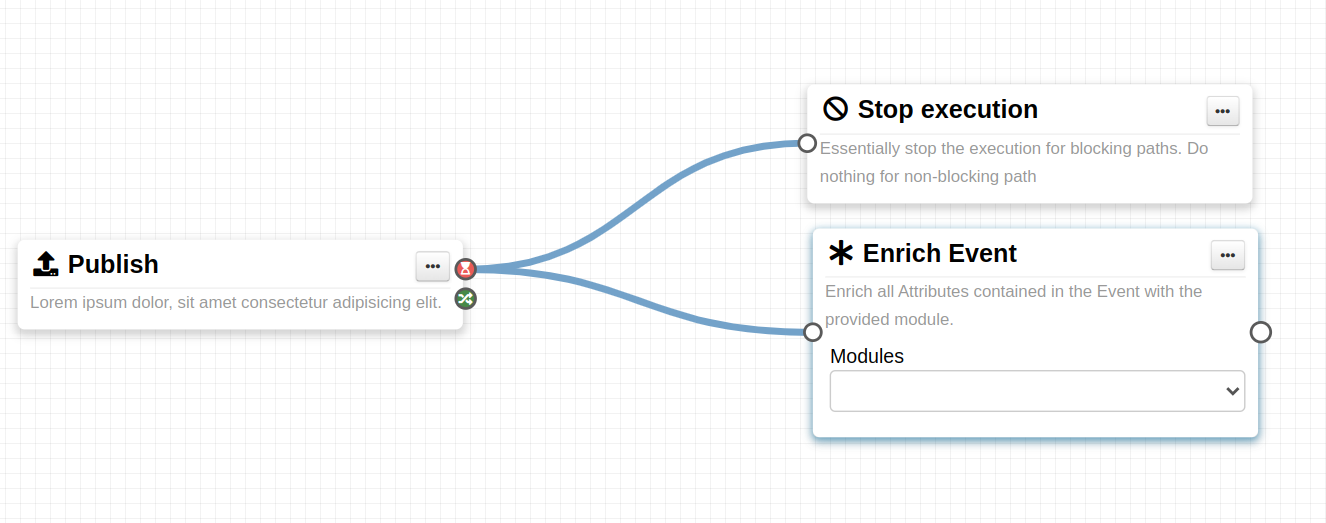
\includegraphics[width=0.9\linewidth]{pictures/example-4.png}
    \end{center}
    \begin{enumerate}
        \item Will \texttt{Enrich Event} module be executed?
        \begin{itemize}
            \item \textbf{Yes} and \textbf{No}. The execution order for the same output is not guaranteed
            \item If \texttt{Stop execution} is executed first, it's a no.
        \end{itemize}
    \end{enumerate}
\end{frame}

\begin{frame}
    \frametitle{Workflow example 5}
    \begin{center}
        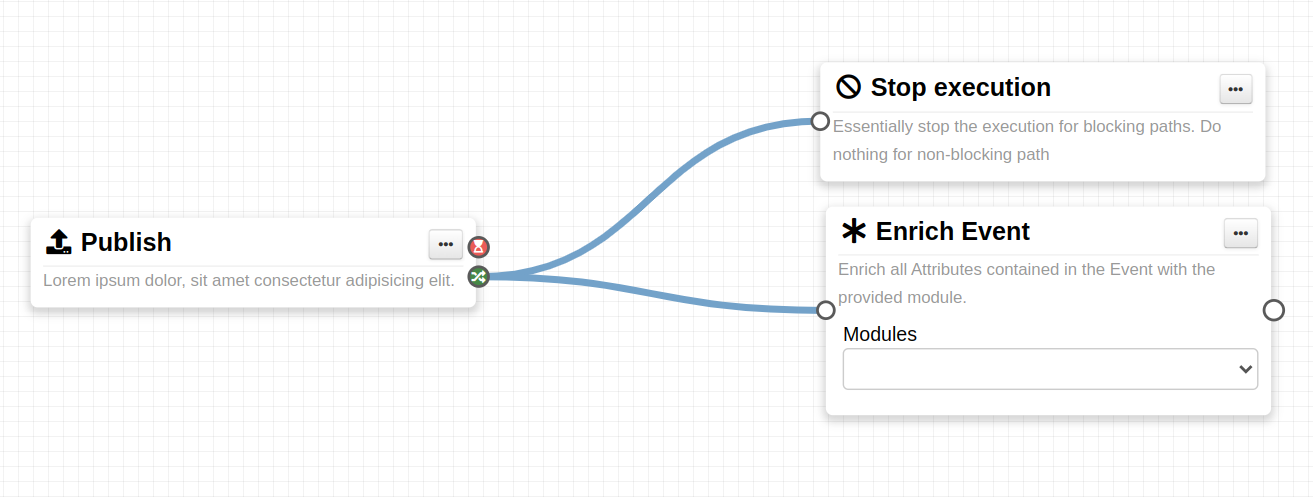
\includegraphics[width=0.9\linewidth]{pictures/example-5.png}
    \end{center}
    \begin{enumerate}
        \item Will \texttt{Enrich Event} module be executed?
    \end{enumerate}
\end{frame}
\begin{frame}
    \frametitle{Workflow example 5: Answers}
    \begin{center}
        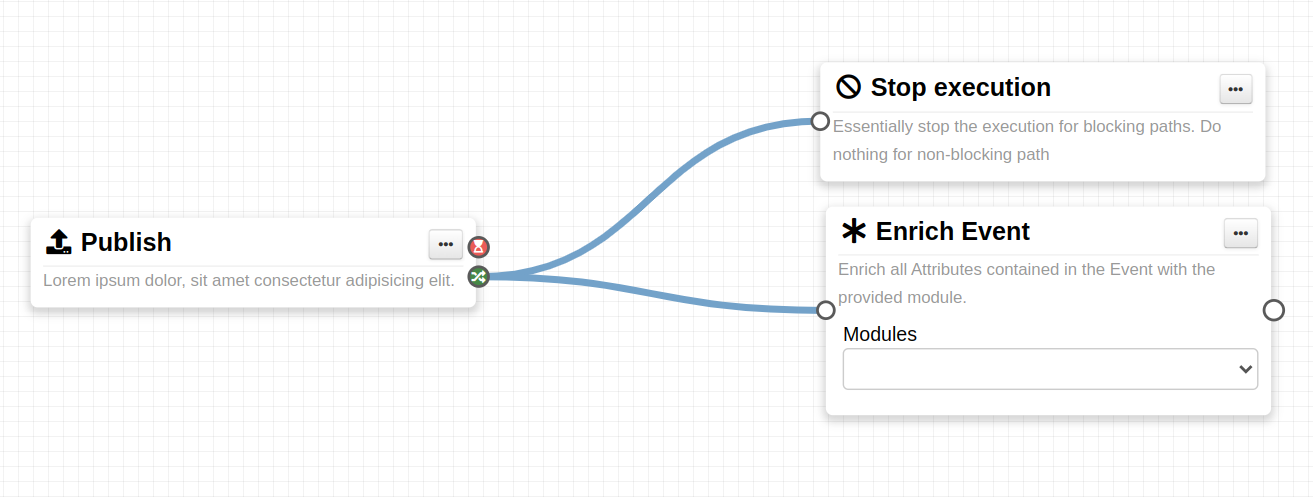
\includegraphics[width=0.9\linewidth]{pictures/example-5.png}
    \end{center}
    \begin{enumerate}
        \item Will \texttt{Enrich Event} module be executed?
        \begin{itemize}
            \item \textbf{Yes}. The execution order for the same output is not guaranteed
            \item However, as we are in a non-blocking path, the outcome of the execution of another path has no impact
        \end{itemize}
    \end{enumerate}
\end{frame}

\begin{frame}
    \frametitle{Workflow example 6}
    \begin{center}
        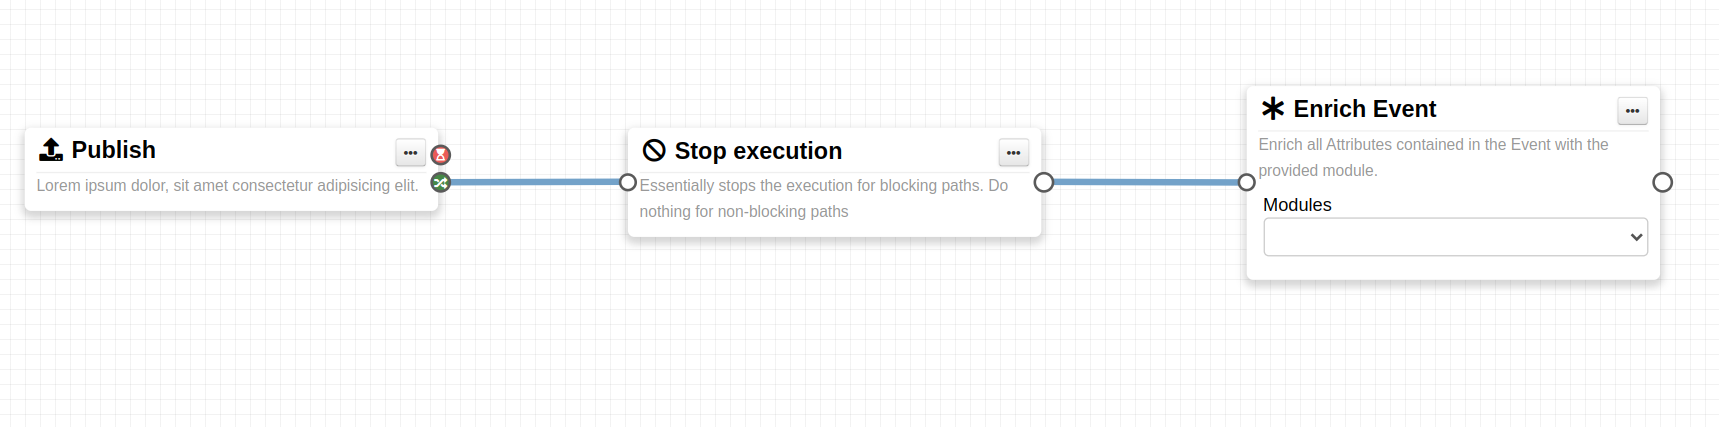
\includegraphics[width=0.9\linewidth]{pictures/example-6.png}
    \end{center}
    \begin{enumerate}
        \item Will \texttt{Enrich Event} module be executed?
    \end{enumerate}
\end{frame}
\begin{frame}
    \frametitle{Workflow example 6: Answers}
    \begin{center}
        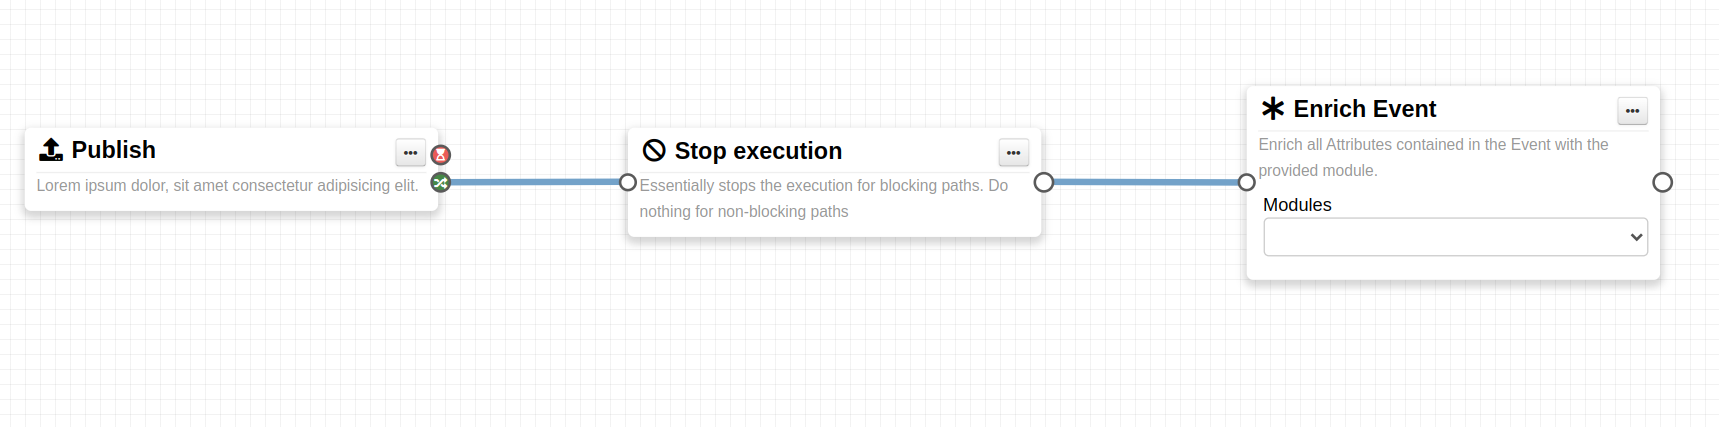
\includegraphics[width=0.9\linewidth]{pictures/example-6.png}
    \end{center}
    \begin{enumerate}
        \item Will \texttt{Enrich Event} module be executed?
        \begin{itemize}
            \item \textbf{No}. Even if we are in a non-blocking path, if the current execution path is blocked, the execution will be stopped
        \end{itemize}
    \end{enumerate}
\end{frame}

\begin{frame}
    \frametitle{Workflow example 7}
    \vspace{-2em}
    \begin{center}
        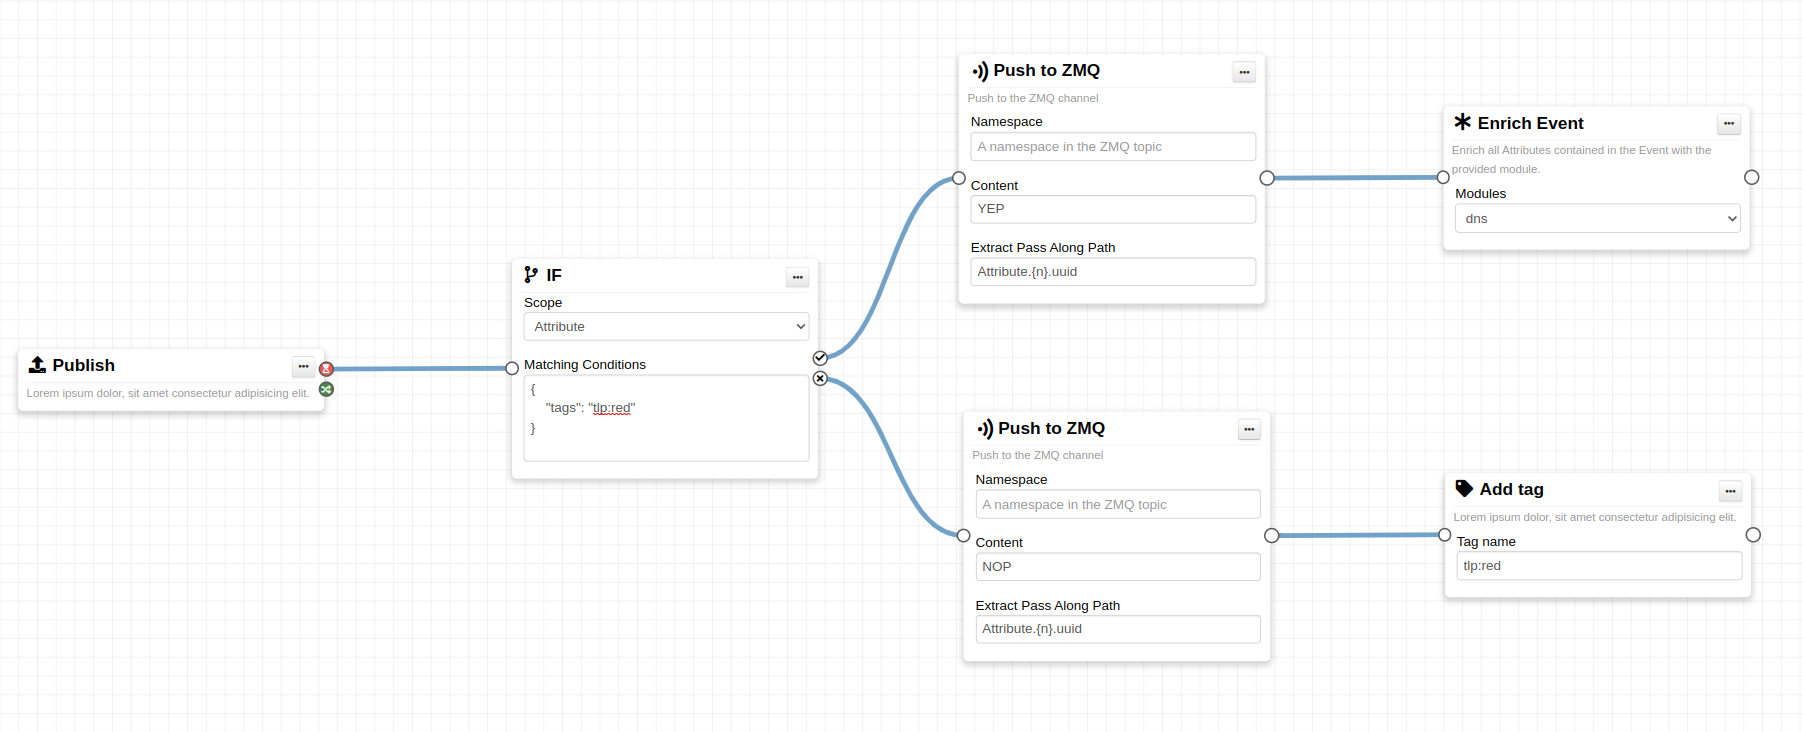
\includegraphics[width=1.05\linewidth]{pictures/example-7.png}
    \end{center}
    \begin{center}
        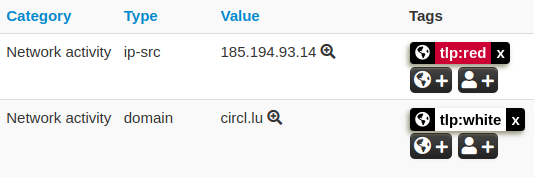
\includegraphics[width=0.45\linewidth]{pictures/event-1.png}
    \end{center}
    \begin{enumerate}
        \item Will \texttt{Enrich Event} module be executed?
        \item Will \texttt{circl.lu} have a tag attached to it?
    \end{enumerate}
\end{frame}
\begin{frame}
    \frametitle{Workflow example 7: Answers}
    \begin{center}
        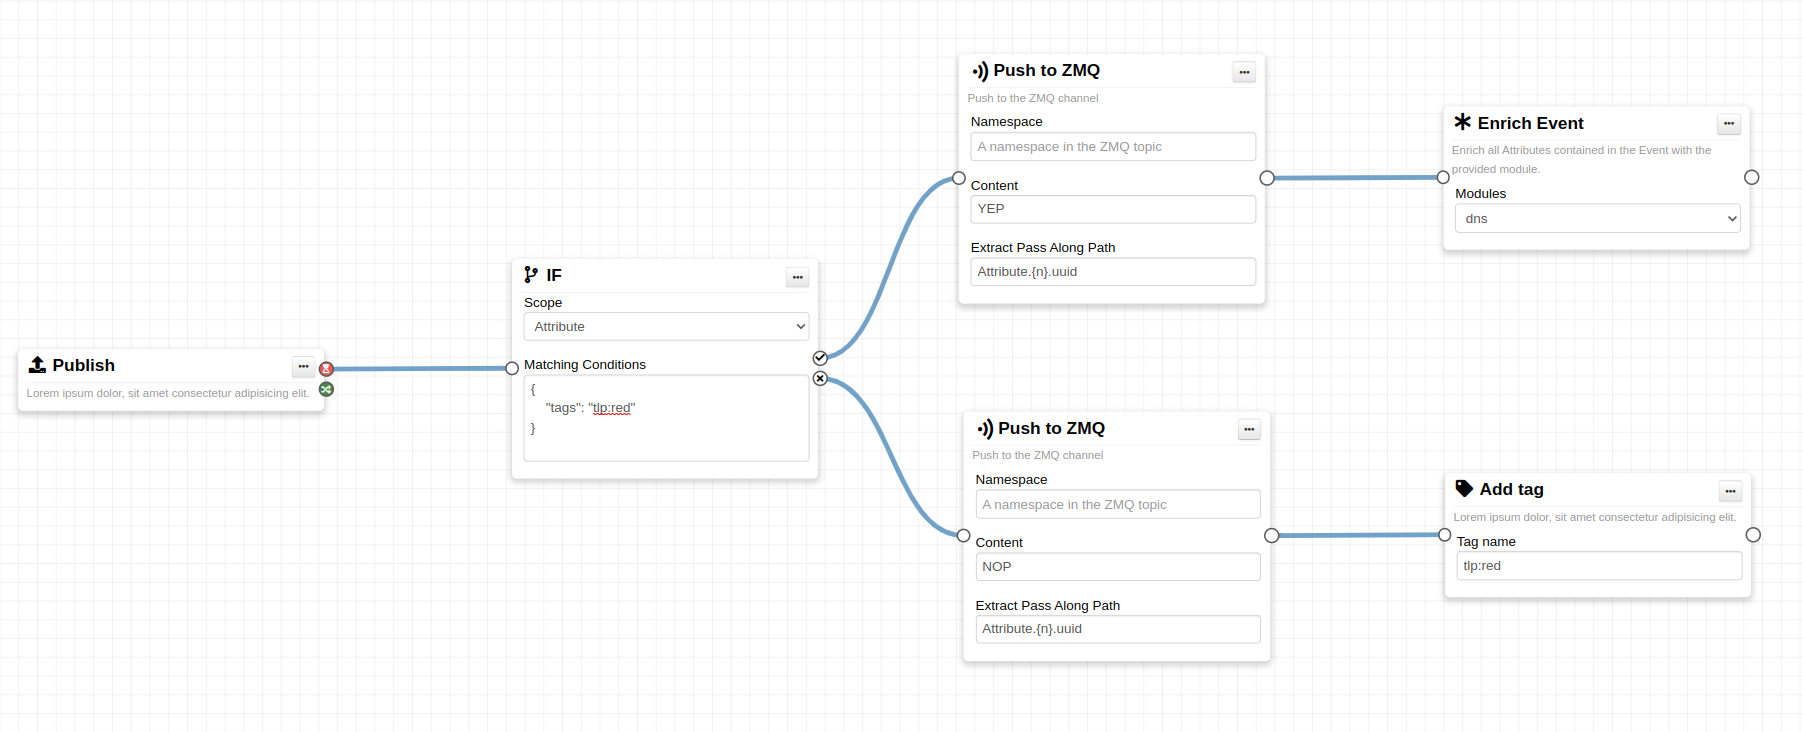
\includegraphics[width=0.7\linewidth]{pictures/example-7.png}
    \end{center}
    \begin{center}
        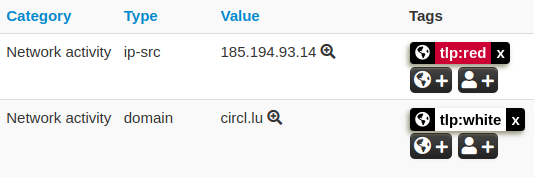
\includegraphics[width=0.3\linewidth]{pictures/event-1.png}
    \end{center}
    \begin{enumerate}
        \item Will \texttt{Enrich Event} module be executed?
        \begin{itemize}
            \item \textbf{Yes}. The event contains an attribute satisfying the matching condition
        \end{itemize}
        \item Will \texttt{circl.lu} have a tag attached to it?
        \begin{itemize}
            \item \textbf{No}. The event contains an attribute satisfying the matching condition. The \texttt{else} part will not be executed.
        \end{itemize}
    \end{enumerate}
\end{frame}

